\section{Metod}
Nedan beskrivs hur vi arbetar i gruppen samt hur vi kom fram till vald lösningsmetod. 



\subsection{Vår lösning}
I algoritm~\ref{alg:quadoptsolver} nedanför visas pseudokod för vår implementering av Active set method algoritmen från \emph{Numerical Optimization}.

\begin{algorithm}[H]
\caption{Quadopt-solver}
\label{alg:quadoptsolver}
\begin{algorithmic}
\Procedure{Quadopt-solver}{$problem$ $P$}
\If{$P$ has not feasible starting point $z_0$}
	\State Compute a feasible starting point $z_0$;
\EndIf	
\State Set $activeSet$ to be a subset of the active constraints at $z_0$ in $P$;
\While{$\textbf{true}$}
	\State Solve subproblem to find step direction $p$;
	\If{$p$ is zero vector}
		\If{$activeSet$ has zero constraints}
			\State \textbf{break};
		\EndIf		
		\If{Could not remove constraints from $activeSet$}
			\State \textbf{break};
		\EndIf
	\Else
		\State Take step to better feasible point $z$ in $P$;
		\If{Could not step}
			\State \textbf{break};
		\EndIf
		\State Set $activeSet$ with new active constraints at $z$;	
	\EndIf
\EndWhile
\State  $solution$ in $P\gets z$;

\State \textbf{return} $solution$ in $P$;
	
\EndProcedure
\end{algorithmic}
\end{algorithm}

Som man ser i pseudokoden ovan är vissa delar relativt vaga. Till exempel ''Compute feasible point'' och ''Solve subproblem''. Dessa delar kommer att beskrivas mer i detalj senare, men först tas några av grundstenarna upp.

\subsubsection{Problem}
''Problem''-strukturen (inparametern P i pseudokoden i Algoritm 1) är som namnet säger en struktur för att lagra det kvadratiska problemet, och därmed alla dess parametrar. Parametrarna i fråga är bland annat problemets bivillkor, målfunktion och aktiva mängden bivillkor.

\subsubsection{Working set}
''Working set'' är den struktur som implementerats för att kunna hålla koll på vilka bivillkor som aktiva (activeSet i Algoritm 1). Strukturen är egentligen endast en mängd utav tal där varje tal representerar bivilkorets postion i den totala uppsättningen av bivillkor. Till denna struktur finns det olika funktioner för att modifiera mängden, bland annat ''append'' som lägger till ett element, ''remove'' som tar bort ett element, och ''clear'' som tar bort alla element.


\subsection{Matrisbibliotek}
För att kunna utföra projeket så behövdes det ett matrisbibliotek för att kunna hantera alla matrisoperationer som lösaren behövde göra. Dessa operationer var:
\begin{itemize}

\item addition
\item subtraktion
\item multiplikation
\item beräkna determinat
\item beräkna invers
\item lösa linjära ekvationssystem
\item gausselimination
\item transponering
\item skalärmultiplikation
\item radoperationer
\item kolumnoperationer

\end{itemize}


\subsubsection{Befintliga matrisbibliotek}
Det fanns många bibliotek som hade dessa operationer dock så uppfyllde inget alla krav vi ställde. Vi vill att biblioteket skulle:
\begin{enumerate}
\item ha lättanvänt api
\item prestera bra
\item vara platformsoberoende
\item vara lätt att kompilera
\item ta upp lite minne
\item ha bra dokumenterad kod så man själv kan implementera förbättringar
\end{enumerate} 
De bibliotek som vi undersökte var:
\begin{itemize}

\item GNU Scientific library
\item LAPACK
\item ATLAS
\item NAG

\end{itemize}
GNU gick bort för det krävde att man installera det som ett extern paket vilket vi inte vill att vår kund ska behöva göra. Bortsett från detta så var detta det bibliotek som var mest lovande. 
LAPACK krävde en FORTRAN kompilator för att kunna kompileras och eftersom det var skrivet i FORTRAN så var alla funktionsnamn endast 6 karaktärer vilket inte kan klassas som ett lättanvändt api.
ATLAS bygger på LAPACK så det har ärvt mycket av alla funktionsnamn.
NAG är det modernaste av bibliotekten men även det använder funktionsnamn med 6 karaktärer samt så var dokumentationen sparsam. 
\newline
\newline
Först så övervägdes att göra att API till något av biblioteken för att göra det mer lättanvänt men sedan så bestämdes det att vi skulle göra att eget biblioteket. Anledning till detta var att man då kunde bygga allting på standard c-bibliotek så man inte krävde några externa bibliotek. Detta leder till att biblioteket kunde användas på alla platformar så länge det hade en c-kompilator. 


\subsubsection{matLib}
Namnet på biblioteket valdes till matLib från \textbf{mat}rix \textbf{Lib}rary. Grundtanken med det hela skulle vara att det bara bygger på standard c-bibliotek för att göra det platform oberoendo. Detta har lett till att det även kan användas på till exempel microkontrollers såsom Atmega 2560 eller liknande.
Det var även krav på att det skulle vara ett lättanvänt API så funktionsnamnen var tvugna att vara självförklarade vad funktionen gör. Här är namnen på ett urval av funktionerna:
\lstinputlisting[language=C]{tex/functions.c}

\subsubsection{Implementation}

\subsubsection{Datastrukturer}

\subsection{Kundkontakt}
Projektets kund var som tidigare nämnt industridoktoranden Daniel Simon vid Linköpings Universitet. Kundkontakten kom igång sent på grund av att kunden inte var på Universitetet när projektet drog igång. Vi hade därefter flera möten bara för att förstå vad kunden hade för krav på oss. Någon som var bra var att han hade väldigt bra koll på vad han ville få ut av projektet och han hade redan satt upp de krav som han tyckte var viktigast. Det enda dokument som han tyckte var viktigt att ha insikt i var kravspecifikationen, resterande dokument som rörde projeketet ville han inte ha del utav. Vi iterarade fram en kravspecifikation tillsammans och efter några iterationer så var båda parterna nöjda. Därefter så hade vi inte så mycket kontakt tills dess att vi kom till en punkt där vi behövde hans hjälp för att lösa en del problem. Sedan så tog det ett tag till innan vi hade möten igen för det det var mycket jobb innan vi hade fått ihop något som kunde visas upp. 
\newline
\newline
Ett av kraven som vi hade satt upp var att lösaren skulle kunna hantera felaktig indata, detta visade sig efteråt vara onödigt då kunden var säker på att detta in skulle ske så lösaren har inte så många tester för indata. Ett annat krav var att lösaren skulle vara lika snabb eller snabbare än den kommersiella programvaran Gurobi. Detta visade sig senare vara svårare än vad som först var förväntat så detta krav kunde vi förhandla bort med kunden. I slutändan så var han nöjd med produkten. Det han var ute efter var en bra grund att bygga vidare på och koden är väldigt bra dokumenterad och strukturerad så det går definitivt bra att bygga vidare på den. 

\subsection{GUI och parser}
Förutom optimeringsalgoritmen skulle ett GUI (Graphical User Interface) och parser skapas. I GUI:t är det menat att användaren ska fylla in hur problemet ska se och samtidigt deklarera variabler för problemet. Sedan skall parser tolka detta och skapa en C-fil. Se figur \ref{fig:quadoptgui} för att se hur GUI:t ser ut.
\begin{figure}
\centerline{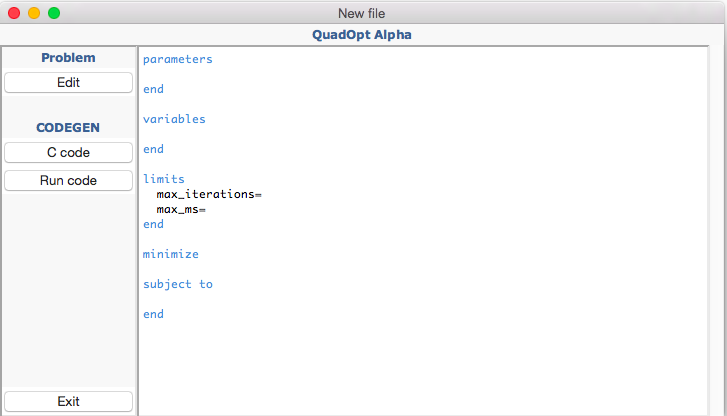
\includegraphics[scale=0.58]{grafik/QuadOptGUI}}
\caption{QuadOpt GUI}
\label{fig:quadoptgui}
\end{figure}
GUI:t skapades med hjälp av språket Python och tkinter. Anledningen till att språket Python användes var för att alla i kandidatgruppen har erfarenhet av språket samt att språket är plattformsoberoende. Visserligen är Java också ett plattformsoberoende språk som det diskuterades om att använda, men alla i kandidatgruppen hade inte erfarenhet av språket och valet föll på Python.
\newline
\newline
Tkinter är ett grafiskt bibliotek, dvs ett bibliotek som hjälper till att forma ett GUI. Anledningen till att Tkinter användes var för att det är lätt att använda och det är ett standardbibliotek som är det mest använda inom Python.
\newline
\newline
HÄR SKA DET STÅ LITE SAKER OM PARSERN. 

\subsection{Lösaren i MATLAB}
För att kalla på lösaren från MATLAB användes MEX. Mexfunktionen från figur~\ref{fig:mex} användes i en C fil som döptes till ''quadopt''. I denna fil fanns matrisbiblioteket och våran lösare importerad. Först görs alla inskickade MATLAB matriser om till matriser från matrisbiblioteket genom att iterera över ''prhs[]'' och skicka MATLAB matrisernas rader och kolumner till ''create\_matrix''. De konverterade matriserna läggs i problem strukten och skickas till lösaren. Den resulterande matrisen konverteras till en MATLAB matris och läggs i ''plhs[0]''.

\subsection{Utvecklingsmetod}
Under projektets gång har det inte funnits någon uppenbar utvecklingsmetodik som kandidatgruppen har följt. Inledningsvis i projektet diskuterades att vissa egenskaper från någon utvecklingsmetodik skulle följas, detta tas upp i underkapitlet ''Förstudien''. När iteration 1 påbörjades fanns det ingen självklar utvecklingsmetodik som följdes, men växte fram under projektets gång och detta tas upp i underkapitlet ''Resterande iterationer''.
\newline
\newline
För att sammanfatta hur kandidatgruppen arbetade, så  inleddes en normal arbetsvecka med möte för att stämma av hur det går för alla i gruppen, om de har förekommit några problem och vad som bör göras härnäst. För att sedan arbeta med de ''practices'' från ''eXtreme programming'' och fullfölja de aktiviteter som satts upp under förstudien. 
\newline
\newline%
Kandidatgruppen har även haft en egen hemsida som innehåller en kalender och i denna kalender brukar möten och arbetspass bokas in så medlemmar kan strukturera upp hur deras vecka ser ut.


\subsubsection{Förstudien}
Under förstudien i detta kandidatprojekt var gruppmedlemmarna överens om att någon sorts utvecklingsmetodik skulle finnas till hands. Det mest naturliga valet var att använda sig av utvecklingsmetodiken ''Scrum'', då flertalet medlemmar i gruppen har tidigare erfarenhet av den. ''Scrum'' är ett agilt arbetssätt för projekt, metodiken används främst i mjukvarusammanhang, men kan även användas för projekt med annan inriktning. https://www.scrumalliance.org/why-scrum
\newline
\newline
Planen var att inte att använda sig av alla attribut som ''Scrum'' har att erbjuda, utan att plocka ut de bästa delar, då vissa attribut kan kännas lite överflödiga. Den viktigaste attributen som hade beräknats att ta med från ''Scrum'' var det såkallade ''Scrum table''. En ''Scrum table'' är helt enkelt en tavla som i vårt fall skulle innehålla tre kategorier, dessa syns nedan.
\begin{itemize}
  \item "Ej påbörjade"
  \item "Under arbete"
  \item "Klart"
\end{itemize}
Under varje kategori skulle sedan ett antal aktiviteter finnas med. Dessa aktiviteter skulle känneteckna det som behövdes göras för att projektet skulle bli klart. Varje aktivitet hade en tidsstämpel som antydde hur lång tid det bör ta att utföra aktiviteten. Ett exempel kan vara att en person ser att aktiviteten ''Implementera matrisaritmetik'' finns under kategorien ''Ej påbörjade''. Den aktiviteten har en tidsstämpel på 20 timmar, dvs det beräknas ta 20 timmar att implementera matrisaritmetik. Om personen vill arbeta med denna aktivitet skulle han/hon flytta denna aktiviteten till kategorien ''Under arbete'' för att sedan flytta den till ''Klart'' när aktiviteten är klar. Antalet timmar för varje aktivitet bestämdes genom diskussion, men främst gissningar då gruppen inte hade tidigare erfarenhet av någon av dessa aktiviteter sen tidigare.
\newline
\newline
Den andra attributen som hade planerats ta med från ''Scrum'' var även ett ''Burn down chart'', dvs en graf som visar hur mycket jobb som finns kvar att göra i jämförelse med hur mycket tid som finns kvar. Detta är lätt att implementera då tavlan nämnd tidigare skulle hålla kolla på timmar på ett strukturerat sätt. 
\newline
\newline
Detta var alltså planen, att implementera en variant av ''Scrum'' med huvudattribut ''Scrum table'' och ''Burn down chart''. För att implementera detta användes ett antal mjukvaruapplikationer. Den första applikationen som användes var ''Trac'', en webbapplikation som används för utveckling av mjukvaruprojekt. ''Trac'' hade de attribut som ''Scrum table'' och ''Burn down chart'', men det var  inget lätt system att förstå och omständigt att konfigurera. Ingen i kandidatgruppen ansåg att ''Trac'' var tillräckligt bra och värt att lägga ytterligare tid på, därav användes inte det. Sedan gavs ''Trello'' en chans, ''Trello'' är också en webbapplikation, men dess huvudsyfte är att visa ett ''Scrum table''. Aktiviteterna i ''Trello'' gick inte att lägga timmar på och ett ''Burn down chart'' fanns inte heller tillgängligt, åtminstone inte utan använda sig av externa program. Medlemmarna i kandidatgruppen installerade externa program för att få dessa funktioner att funka, men precis som med ''Trac'' kändes systemet för alldeles krångligt och inte heller värt att lägga tid på. Se figur \ref{fig:trello} för en bild på hur ''Trello'' såg ut för kandidatgruppen.

\begin{figure}[h]
\centerline{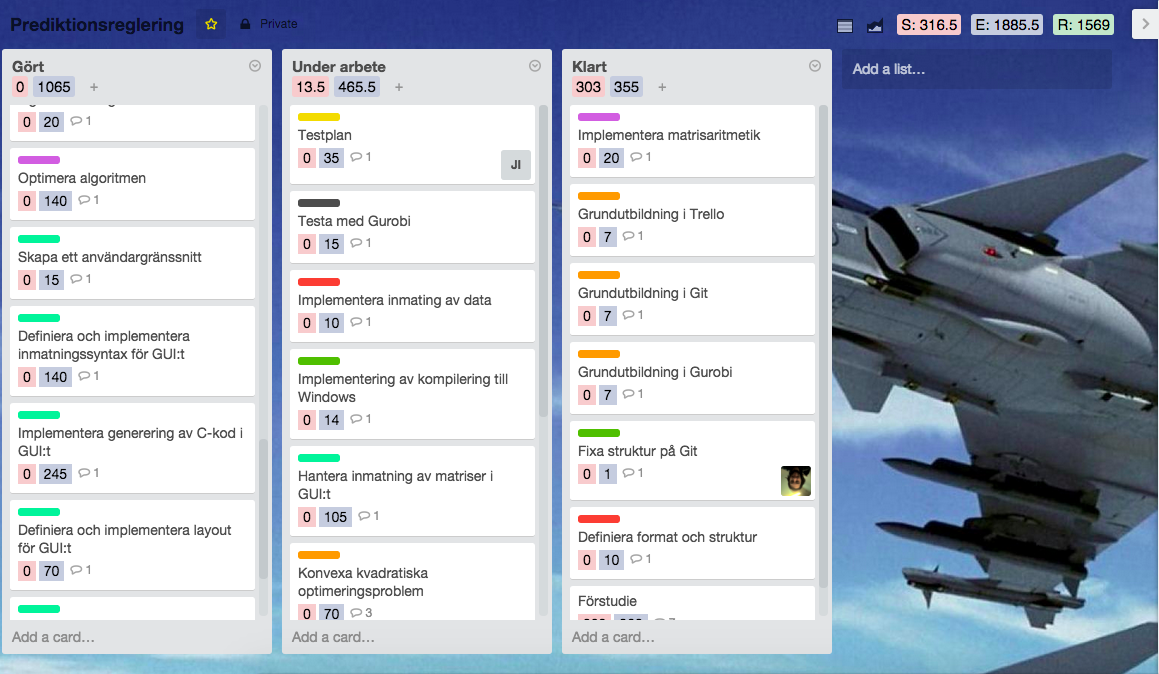
\includegraphics[scale=0.3]{grafik/trello}}
\caption{Scrum table i Trello}
\label{fig:trello}
\end{figure}

\noindent Efter dessa försök med ''Trac'' och ''Trello'' gav kandidatgruppen upp med tanken av att använda utvecklingsmetodiken ''Scrum'' och inledde första iterationen av projektet utan någon specifik utvecklingsmetodik.
\textcolor{red}{ hade det funkat med en whiteboardtavla?}.

\subsubsection{Resterande iterationer}
Som nämnt gick kandidatgruppen in i första iterationen utan någon specifik utvecklingsmetodik, men under arbetetsgången växte en sorts utvecklingsmetodik fram.
\newline
\newline
Under projektet arbetade samtliga gruppmedlemmar i närheten av varandra. I ett tidigt skede hade gruppen tillgång till ett kontor där arbetet kunde genomföras samt möten kunde hållas. Genom att arbeta så nära varandra underlättade det att hjälpa till där det behövdes och om ett problem uppstod kunde det snabbt tas itu med.
\newline
\newline
Den utvecklingsmetodik som växte fram för kandidatgruppen kan efterlikna utvecklingsmetodiken ''eXtreme programming'' också kallad XP. XP är likt ''Scrum'', ett agilt arbetssätt för mjukvaruprojekt. XP innehåller ett antal ''practices'', dvs metoder för hur man ska behandla kod. De metoder som förekommer i kandidatgruppen, finns listade nedan.
\begin{itemize}
  \item \textbf{Pairprogramming} - I kandidatgruppen har vissa medlemmar parprogrammerat. Detta innebär att två stycken personer ska utföra en uppgift, en skriver kod och den andra granskar. Ett byte av roller sker också emellanåt. Genom att parprogrammera kan man diskutera om vad som skulle ge upphov till den bästa lösningen.
  \item \textbf{Refactoring} - ''Refactoring'' är något som har dykt upp väldigt mycket under arbetsgången. Poängen med ''Refactoring'' är att förbättra kods läsbarhets samt reducera komplexiteten utan att ändra kodens syfte. Detta har varit en stor del av projektet då kunden har tryckt på att kod ska vara väldokumenterad och strukturerad.
<<<<<<< HEAD
  \item \textbf{Continuous integeration} - ''Continuous integration'' eller CI som det brukar kallas har också varit en stor del av kandidatprojektet. Det är väldigt viktigt att all kod som skrivs funkar med de olika komponenterna i detta projekt, t.ex. att matrisbiblioteket och koden för lösaren funkar tillsammans. Det som har gjorts i projektet är att tester skrivs för de allra viktigaste funktioner och dessa testas kontinuerligt genom att använda ''Travis CI''. ''Travis CI'' kompilerar all kod och säger till om testerna misslyckas eller inte. CI står för kontinuerlig integration.
=======
  \item \textbf{Continuous integeration} - ''Continuous integration'' eller CI som det brukar kallas har också varit en stor del av kandidatprojektet. Det är väldigt viktigt att all kod som skrivs funkar med de olika komponenterna i detta projekt, t.ex. att matrisbiblioteket och koden för lösaren funkar tillsammans. Det som har gjorts i projektet är att tester skrivs för de allra viktigaste funktioner och dessa testas kontinuerligt genom att använda ''Travis CI''. ''Travis CI'' kompilerar all kod och säger till om testerna misslyckas eller inte. CI översatt till svenska står för kontinuerlig integration.
>>>>>>> db745441f056e458967f2d001513df66b167c743
\end{itemize}
Med hjälp av dessa ''practices'' och god kommunikation mellan gruppmedlemmarna kunde projektet genomföras. 

\subsubsection{SEMAT Kernel}
SEMAT står för Software Engineering Method and Theory och är ett iniativ för att förbättra mjukvaruutvecklingsindustrin. Med olika verktyg är det tänkt att ledare och managers ska kunna ge sina utvecklare bättre förutsättningar för att bli bättre, snabbare, billigare och gladare. \citep{semat} 
\newline
\newline
Ivar Jacobson, som är en av grundarna till SEMAT, har utvecklat ett verktyg kallat Alpha State. Alpha States representerar olika faser ett mjukvaruprojekt kan gå igenom.
\newline
\newline 
Under kandidatprojektet har Alpha States använts i form av Alpha State Cards. På korten finns alla faser och de krav som ska vara uppfyllda för just den fasen. Genom att checka av vilka krav som är uppfyllda för vilken fas kan gruppen få ökad förståelse för vilket tillstånd projektet befinner sig i.  

\subsubsection{Utvecklingsverktyg}
De verktygen som användes under detta kandidatprojekt var främst
\newline
\newline
\textbf{Virtuell maskin.} Till kandidatgruppens förfogande fanns en virtuell maskin med 8 gb hårddisk, 1 gb RAM och 1 gb swap. Den kör Debian GNU/Linux Stable (Wheezy). Maskinen används främst för att ''hosta'' kandidatgruppens hemsida. Hemsidan består av nyttiga länkar och en kalender som i sin tur består av möten och grupparbeten som gruppmedlemmar bör medverka i.
\newline
\newline 
\textbf{Git.} Git är ett versionshanteringssystem. Ett versionshanteringssystem möjliggör gör parallell utveckling och håller koll på versioner av ens projekt i linjär tid. Med hjälp av Git har kandidatgruppen kunnat arbeta parallellt med stora delar av kod samt har individer som har velat jobba med något experimentellt kunnat gå sin egen väg genom att skapa en branch och jobba på den branchen. Det brukar finns en master branch, dvs där det huvudsakliga arbetet görs och sen kan man skapa andra branches för kod annat. 
\newline
\newline 
\textbf{Github.} Github är ett webbhotell som använder Git. Här kan man lagra alla versioner av sin kod. Kandidatgruppen lagrar alla väsentligt dokumentation för projektet på Github, dvs alla dokument som skrivs och all kod. Kandidatgruppens Github är dessutom privat så bara folk som ska ha med dokumentationen att göra har tillgång till sidan.
\newline
\newline
\textbf{Byggsystem.} Ett byggsystem av kandidatgruppen har skapats och gruppen klassar det som ett utvecklingsverktyg. Byggsystemet kompilerar all kod och kör alla tester som finns i biblioteket. Detta har underlättat arbetsprocessen enormt, då efter man har skrivit kod kan man helt enkelt skriva in make i terminalen och då kompileras allt och alla tester. Byggsystem är utvecklat i språket Make.
\newline
\newline 
\textbf{Travis CI.} Travis CI är en byggserver som används tillsammans med Github. Det Travis gör är att kalla på byggsystemet som sedan kompilerar all kod och kör testfilerna. Travis säger till om koden är kompilerbar eller ej, om den är kompilerbar så kör Travis alla tester som finns och säger till om testerna lyckades eller inte. Om Travis inte skulle ha lyckats kompilera koden eller klara alla tester så ändrar Travis statusen på projektet till ''build failing'' vilket visas på kandidatgruppens Github-sida. Om den klara allt så visar den ''build passing''. Den som lägger upp ny kod och orsakar en ''build failing'' får ett e-mail om att koden som har lagts upp inte är okej.
\newline
\newline
\textbf{Valgrind.} Lösaren allokerar mycket minne och d denna är implementerad i C så måste man själv se till att frigöra allt minne. För att vara säkra på att det inte fanns några minnesläckor så användes Valgrind. Hittades några minnesläckor så ǻtergärdades dessa.  
\newline
\newline
\textbf{Emacs}. Under projektet användes ett flertal olika editorer för att skriva kod. En av dem var Emacs som är en textredigerare skapad Richard 	Stallman. Vissa i kandidatgruppen använde emacs då de uppskattade att man enkelt kan arbete med flera filer vid sidan om varandra samt lättheten att byta mellan filer.
\newline
\newline
\textbf{Sublime Text.} Sublime är en annan textredigerare som vissa i gruppen använde. Det som är utmärkande drag för Sublime är att redigeraren har en rätt så unik syntax-highlighting, dvs hur den belyser text. Detta uppskattades samt att inlärningsprocessen var enkel.s
\newline
\newline
\textbf{Eclipse.} Eclipse är ingen texteditor utan en IDE, dvs en integrerad utvecklingsmiljö. Den innehåller en textredigerare, kompilator och debugger. De som använde Eclipse tyckte att debuggern kom tillhands väldigt ofta och därför använde de Eclipse.
\newline
\newline
\textbf{Matlab.} Matlab är ett datorprogram och programspråk som främst används för tekniska beräkningar och matematiska. Eftersom optimeringsalgoritmen som skrevs skulle kunna användas i Matlab har Matlab varit ett viktigt verktyg för kandidatgruppen. Tester av gruppens optimeringsalgoritm har gjorts i Matlab många gånger. Även Matlabs matrisoperationer har varit till stor nytta för kandidatgruppen för att underlätta räkning av uppgifter. Matlab har även en egen optimeringslösare som liknar kandidatgruppens, jämförelser har gjorts med den vid ett flertal tillfällen.
\newline
\newline
\textbf{Gurobi.} Gurobi är ett kommersiellt programverktyg som specialiserar sig att lösa optimeringsproblem utav av alla typer. Kandidatgruppen hade i början ett krav på att vara likvärdig med Gurobi gällande hastighet. Detta har lett till att många tester har gjorts med Gurobi.
\newline
\newline
\textbf{Texmaker.} Texmaker är en textredigerare för att skriva i språket \LaTeX. Alla de dokument som har skrivits under kandidatprojektet har skrivits i {\LaTeX} och då har Texmaker varit till stor hjälp. Anledning till att många i kandidatgruppen har använt Texmaker är för att de funkar på individernas operativsystem.
\newline
\newline
\textbf{Gummi.} Gummi är också en textredigerare för att skriva i språket {\LaTeX} men finns enbart för Linux system. Gummi kan anses vara ett lättviktigare program än Texmaker som är lite tyngre och har funktioner som inte har varit så nödvändiga.
\newline
\newline
\textbf{Google Drive.} Google Drive har använts under projektets gång för att arbete med dokument med mindre betydelse. Dokument som mötesrapporter och tidsrapporter som enbart är menat för kandidatgruppen och handledare. Vid presentationstillfällen har Google Drive också varit till nytta för att göra presentationer.
\newline
\newline
\textbf{Time Profiler.} Time Profiler är ett verktyg som finns förinstallerad på Mac-datorer. Verktyget kan visa hur mycket tid som spenderas på funktioner i ett program. Då optimeringsalgoritmen som har skapats ska ta så lite tid som möjligt har detta verktyg kommit tillhands för att se hur mycket tid algoritmen spenderar i vissa funktioner. Genom att hitta de funktioner som tar mest tid att utföra har kandidatgruppen kunnat snabba upp dem någorlunda.
\newline
\newline
\textbf{DDD.} Data Diplay Debugger har använts i projektet för att hitta kritiska fel. Felsökningen av kod sker i ett grafiskt användargränssnitt och är ett väldigt kraftfullt verktyg.
\newline
\newline
\textbf{Doxygen.} Doxygen är en dokumentationsgenerator för programvara. Programmet funkar genom att användaren har skrivit kommenterar i koden under projektets gång och då använder Doxygen sig av dessa kommentarer för att generera ett dokument. Resultaten blir en pdf som består av förklaringar för funktioner och datastrukturer. 

\subsection{Forskningsmetod}
Som tidigare nämnt var det tre olika algoritmer som var aktuella för projektet och som alla fanns med och beskrevs i boken Numerical Optimization. Detta avsnitt kommer behandla hur algoritmerna jämfördes mot varandra för att slutligen avgöra vilken som skulle användas.
\newline
\newline
De tre algoritmerna som fanns var \emph{Active set method}, \emph{Gradient Projection method} och \emph{Interior point method}. Dessa algoritmer hade sina egna styrkor och svagheter, och det var just dessa som behövde jämföras utifrån prediktionsregleringsproblemets behov.

\subsubsection{Faktorer}
För att kunna avgöra vilken av algoritmerna som var den bäst lämpade för optimeringsproblemet, så behövdes det ett antal faktorer att jämföra dem emot.

\paragraph{Implementerbarhet}
Olika faktorer som spelade in var bland annat och möjligen det viktigaste implementerbarhet, mest eftersom projektet är väldigt tidsbegränsat och det finns ingen möjlighet till att överskrida tidsbudgeten. Eftersom det även var ett krav att lösaren skulle implementeras i C så var man tvungen att kolla vilka olika möjligheter för implementering som fanns där.

\paragraph{Hastighet}
Hastighet var även en väldigt viktig faktor, just på grund av att ett av de få krav som vi faktiskt hade var att programmet skulle vara lika snabbt eller snabbare än det kommersiella programmet Gurobi som används för att lösa alla möjliga sorters optimeringsproblem. En fördel vi hade gentemot Gurobi var att vår lösaren kunde optimeras för just detta problem och behövde inte vara lika generell som Gurobi.

\paragraph{Skalbarhet}
En annan viktig faktor som var avgörande var skalbarhet. Matrisernas storlekar på problemet som ska lösas kan vara uppemot flera hundra element i båda dimensionerna, därför var det väldigt viktigt att algoritmen hade en tidskomplexitet som inte var allt för stor. Just i början kan detta vara väldigt svårt att veta eftersom det inte finns så stora möjligheter till att testa större problem, utan dessa kan endast testas i ett senare skede när lösaren verkligen kommit så långt att den kan hantera dem.

\paragraph{Komplexitet}
Algoritmerna i sig kan verka vara väldigt snabba och skalbara men kan kräva en massa andra extra förkunskaper för att man ska kunna förstå sig på dem, och som skulle ta alldeles för lång tid för att läsa in inom projektets tidsbudget. Detta hänger delvis ihop med implementerbarhet, eftersom båda har med algoritmens svårighetsgrad att göra.

\paragraph{Stabilitet}
Klarar algoritmen alla olika fall av indata. Vad händer vid till exempel nollfall? Kan man lita på att algoritmen alltid kommer fram till en lösning inom rimlig tid. Hur mycket minne förbrukar algoritmen i förhållande till problemets storlek? %Behöver algoritmen någon data som räknas ut på annat vis för att fungera som den ska?

\subsubsection{Algoritmernas för- och nackdelar}
De tre algoritmerna är specialiseade på kvadratisk optimering. Men skiljer sig en del emot hur snabba de är för olika storlekar på problemen.

\paragraph{Active set method}

\paragraph{Gradient Projection method}


\paragraph{Interior point method}


\subsubsection{Algoritmerna gemtemot varandra}
